\documentclass[12pt,twoside]{article}
\usepackage{setspace}
\usepackage[a4paper,hmargin=2.8cm,vmargin=2.0cm,includeheadfoot]{geometry}
\usepackage{indentfirst}

\usepackage{cite}
\usepackage{amsmath,amssymb,amsfonts}
\usepackage{algorithmic}

\usepackage[]{caption}
\usepackage{subcaption}

\usepackage{tabularx}
\usepackage{longtable}
\usepackage[]{multirow}
\usepackage{array} % to allow vertical alignment in tables
\usepackage{makecell} % allows multi-line tables
\usepackage{enumitem} % better enumeration
%\usepackage{subcaption}

\usepackage{graphicx}
\usepackage{textcomp}
\usepackage{xcolor} % allows defining your own colours
\usepackage{chngcntr} % Make nice counter macros availalble
% 	\counterwithin{figure}{subsection} % Add Section Number to Figure Counter
% 	\counterwithin{table}{subsection} % Add Section Number to Table Counter
% \def\BibTeX{{\rm B\kern-.05em{\sc i\kern-.025em b}\kern-.08em
%     T\kern-.1667em\lower.7ex\hbox{E}\kern-.125emX}}

\usepackage{float} % enable forcing locations with [H], [T]

\usepackage{hyperref} % uncomment after document is finished to hyperlink everything
\hypersetup{
    colorlinks,
    linkcolor={red!50!black},
    citecolor={green!30!black},
    urlcolor={blue!80!black}
}


\begin{document}

%\begin{titlepage}

\newcommand{\HRule}{\rule{\linewidth}{0.5mm}} % Defines a new command for the horizontal lines, change thickness here


%----------------------------------------------------------------------------------------
%	LOGO SECTION
%----------------------------------------------------------------------------------------


\includegraphics[width = 6cm]{./figures/imperial}\\[0.5cm] 

\begin{center} % Center remainder of the page

%----------------------------------------------------------------------------------------
%	HEADING SECTIONS
%----------------------------------------------------------------------------------------

\vspace{1.25cm}
\textsc{\Large Final Report for MEng Individual Project}\\[0.5cm] 
\textsc{\large Department of Bioengineering}\\[0.5cm] 
%----------------------------------------------------------------------------------------
%	TITLE SECTION
%----------------------------------------------------------------------------------------

\HRule \\[0.4cm]

\begin{spacing}{1.5}
{ \LARGE \bfseries Wireless Transmission of Electrochemical Signals for Early Diagnosis of Secondary Traumatic Brain Injury }\\
\end{spacing}

\HRule \\[1.5cm]

%----------------------------------------------------------------------------------------
%	AUTHOR SECTION
%----------------------------------------------------------------------------------------

%\begin{minipage}{0.4\hsize}
%\begin{flushleft} 
\large
\textit{Author:}
Aishwarya Pattar
%\end{flushleft}

%\begin{flushleft} 
\large
\textit{Supervisor:}
Professor Martyn G. Boutelle
%\end{flushleft}


\vspace{5cm}
\small
\textit{Submitted in partial fulfilment of the requirements for the award of MEng in Biomedical Engineering from Imperial College London}

\end{center}

\vspace{2.5cm}
June 2019   \hfill  Word Count: 5721

\vfill % Fill the rest of the page with whitespace



\makeatother


\end{titlepage}

%\begin{abstract}
    % Sentence of two about TBI and secondary TBI
    % Sentence about aim of the project
    % Sentence about the prototype
    % Two sentences about the app
    % Sentence about things that were tested to prove
    % Summarise results/discussion about testing
    % Future improvements
    
%\end{abstract}

%\newpage


\section{Introduction}
Traumatic Brain Injury (TBI) occurs from an impact to the head resulting in an injury to the brain, commonly caused by road traffic accidents and falls \cite{Langlois2006}. The severity of the injury sustained to the brain can range from superficial swelling to oedema and haematomas, with higher severity of the TBI resulting in a higher mortality rate as shown in Table~\ref{table:severity of TBI}. Even if the injury does not result in death, TBI can lead to long term disability and cognitive problems \cite{WorldHealthOrganisation2006}. Approximately 2.5 million people visited the hospital for TBI related symptoms in the US during 2013, of which 56,000 result in death \cite{Taylor2017}. The prevalence of this injury incurs an estimated \$60 billion cost annually to society to cover medical costs and lost productivity \cite{Finkelstein2009}. 

Primary TBI is the damage sustained from the initial impact, whereas secondary TBI occurs from the cascade of biochemical processes following from primary TBI, resulting in damage to the tissue surrounding the primary injury site \cite{Norton2008}. Secondary TBI tends to occur after a delayed period of time in about 30\%-40\% of people who have suffered primary TBI, however whether it occurs is unpredictable and unpreventable \cite{Pagkalos2017}. Secondary effects, such as oedema, hypoxia and ischemia, can lead to neural degeneration and irreversible damage which can cause severe disability or be fatal \cite{Murthy2005}. Hence, it is crucial to diagnose secondary TBI as soon as possible and provide appropriate medication to treat and minimise the damage.

\begin{table}[H]
\centering
\begin{tabular}{||c c||} 
 \hline
 Severity of TBI & Mortality (\%) \\ [0.5ex] 
 \hline\hline
 Mild & \textless 1 \\ 
 Moderate & 2-5 \\
 Severe & 20-50 \\
 \hline
\end{tabular}
\caption{Severity of TBI affecting mortality rates \cite{WorldHealthOrganisation2006}}
\label{table:severity of TBI}
\end{table}

Common methods used to diagnose secondary TBI rely on qualitative analysis. An example is the Glasgow Coma Scale which assesses ocular, verbal and motor responses and assigns a score out of 15. This is then accompanied with a neuroimaging method such as a CT scan \cite{WorldHealthOrganisation2006}. The main disadvantage of these methods is that they are subjective, and it is difficult to identify mild symptoms of TBI which are displayed subtly as non-specific symptoms \cite{Bettermann2012}. Furthermore, these methods only capture information at a specific period in time meaning that if symptoms occur, they will be unobserved until the next appointment. 

Early diagnosis is crucial for the best recovery, and to do so, there is a need to continuously monitor the patient and receive quantitative data for accurate diagnosis. The Boutelle Research Group have been looking into utilising brain signals that are associated with TBI. From the primary injury site, spreading depolarisation (SD) waves propagate into surrounding brain tissue and cause secondary damage. The cells in the injury sites have a high energy demand in order to repolarise the membrane potential, hence the glucose concentration in the extracellular fluid transiently decreases by approximately 18-93$\mu M$. The cells tend to undergo anaerobic respiration, so the extracellular lactate concentration transiently increase by 5-100$\mu M$ \cite{D.2010}. Glucose and lactate have been declared by the International Microdialysis Collaborative Group as the most clinically useful signals for the prognosis of TBI \cite{Hutchinson2015}. Furthermore, during the same transient period, the potassium ion concentration increases \cite{Rogers2017} as shown in Figure~\ref{fig: SD}.

\begin{figure}[t]
\centering
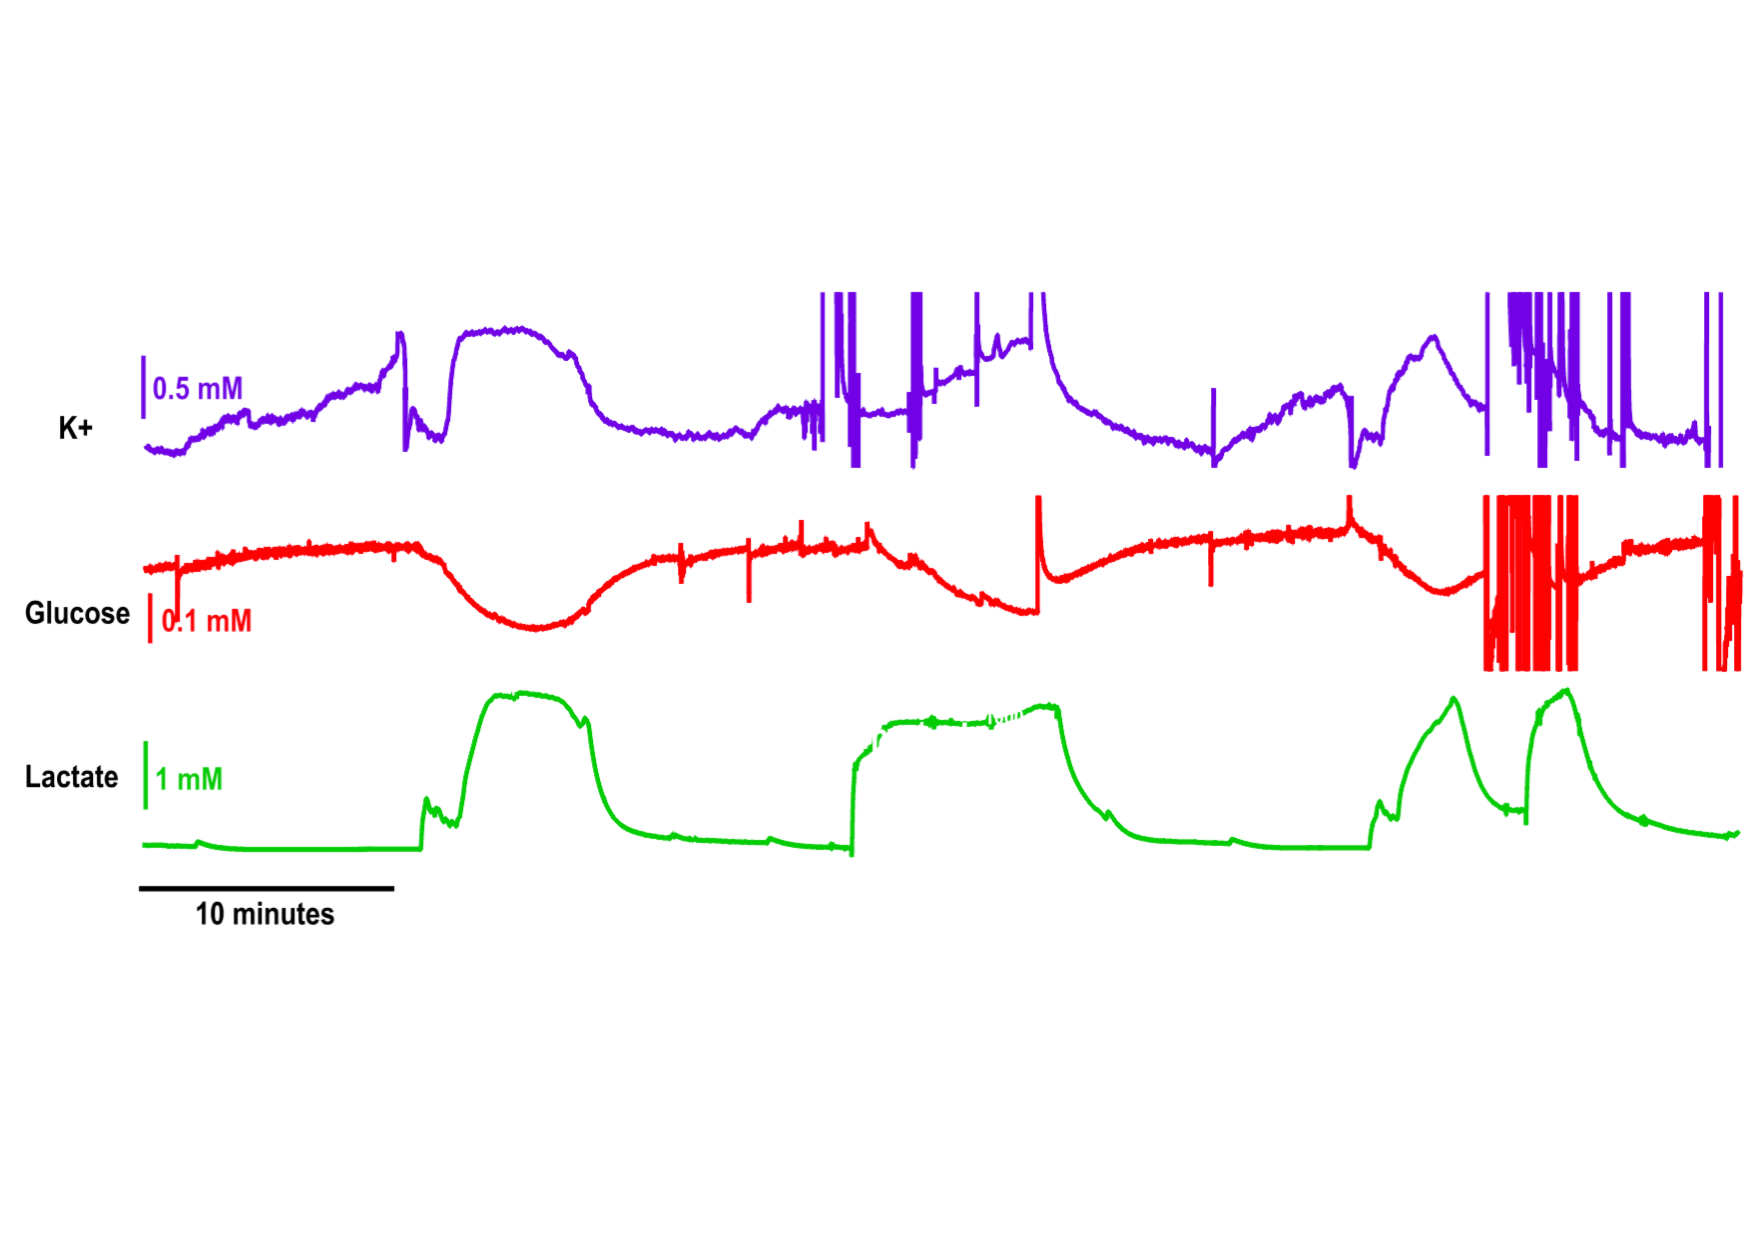
\includegraphics[trim={0cm 5cm 0.5cm  5cm}, clip, width=1\textwidth]{./figures/conc.pdf}
\captionsetup{justification=centering}
\caption{Biochemical changes during an SD occurence at 10 minutes. K+ and lactate show an increase in concentration whilst glucose shows a decrease in concentration \cite{Rogers2017}. Measurements obtained from microdialysis.}
\label{fig: SD}
\end{figure}

The research group have developed implantable diagnostic systems, which can detect these three electrochemical signals of interest, such as the LENBIC \cite{Pagkalos2017}. It contain amperometric channels for the detection of glucose and lactate, and potentiometric channels for the detection of potassium ions from the microdialysis system it is connected to. However, the LENBIC is a wired system, so its limitations include requiring an orifice for the wires to exit the body, the patient's movement is restricted, the wires may break, and the wires may introduce noise \cite{Ferguson2011}. Therefore, a wireless transmission system is more desirable to communicate the electrochemical data. 

\textbf{DOUBLE CHECK WITH MICHELLE ABOUT THIS}
Furthermore, data is extracted from the microdialysis system at the end of experimentation and is later analysed manually by someone who is trained to identify when an SD has occurred. This prevents diagnosis from occurring sooner at the time of the SD. There is a need for the data to be received and analysed in real time to ensure early diagnosis. 

This project aims to develop a wireless communication system between the microdialysis system and an iOS application. Information from the three electrochemical sensors will be received simultaneously in an iPad application in real time. The app must be user friendly and be of high quality as it aims to be used by a clinician to monitor the state of the patient. It is important that the signals are transmitted and displayed accurately so suitable processing methods need to be implemented. 


\newpage

\section{Prototype Design}
The prototype developed intends to be integrated with a PCB currently being developed by the research group. The PCB consists of five potentiometric channels, allowing for the measurement of potassium ion concentration, and four amperometric channels to allow for glucose and lactate concentration measurements. The potentiometric readings are amplified using an instrumental amplifier, and the amperometric readings are amplified using a transimpedance amplifier, which also converts the current to voltage. An ADS1298, which is a 24-bit resolution analogue-to-digital converter (ADC), receives the input measurements simultaneously and discretises and further amplifies the signals \cite{TexasInstruments2010}. An ATmega328p microcontroller is used and the PCB allows for both SPI (serial peripheral interface) and UART (universal asynchronous receiver-transmitter) data transmission capabilities. The PCB design in summarised in the block diagram in Figure~\ref{fig: PCB block diagram}.

\begin{figure}[H]
\centering
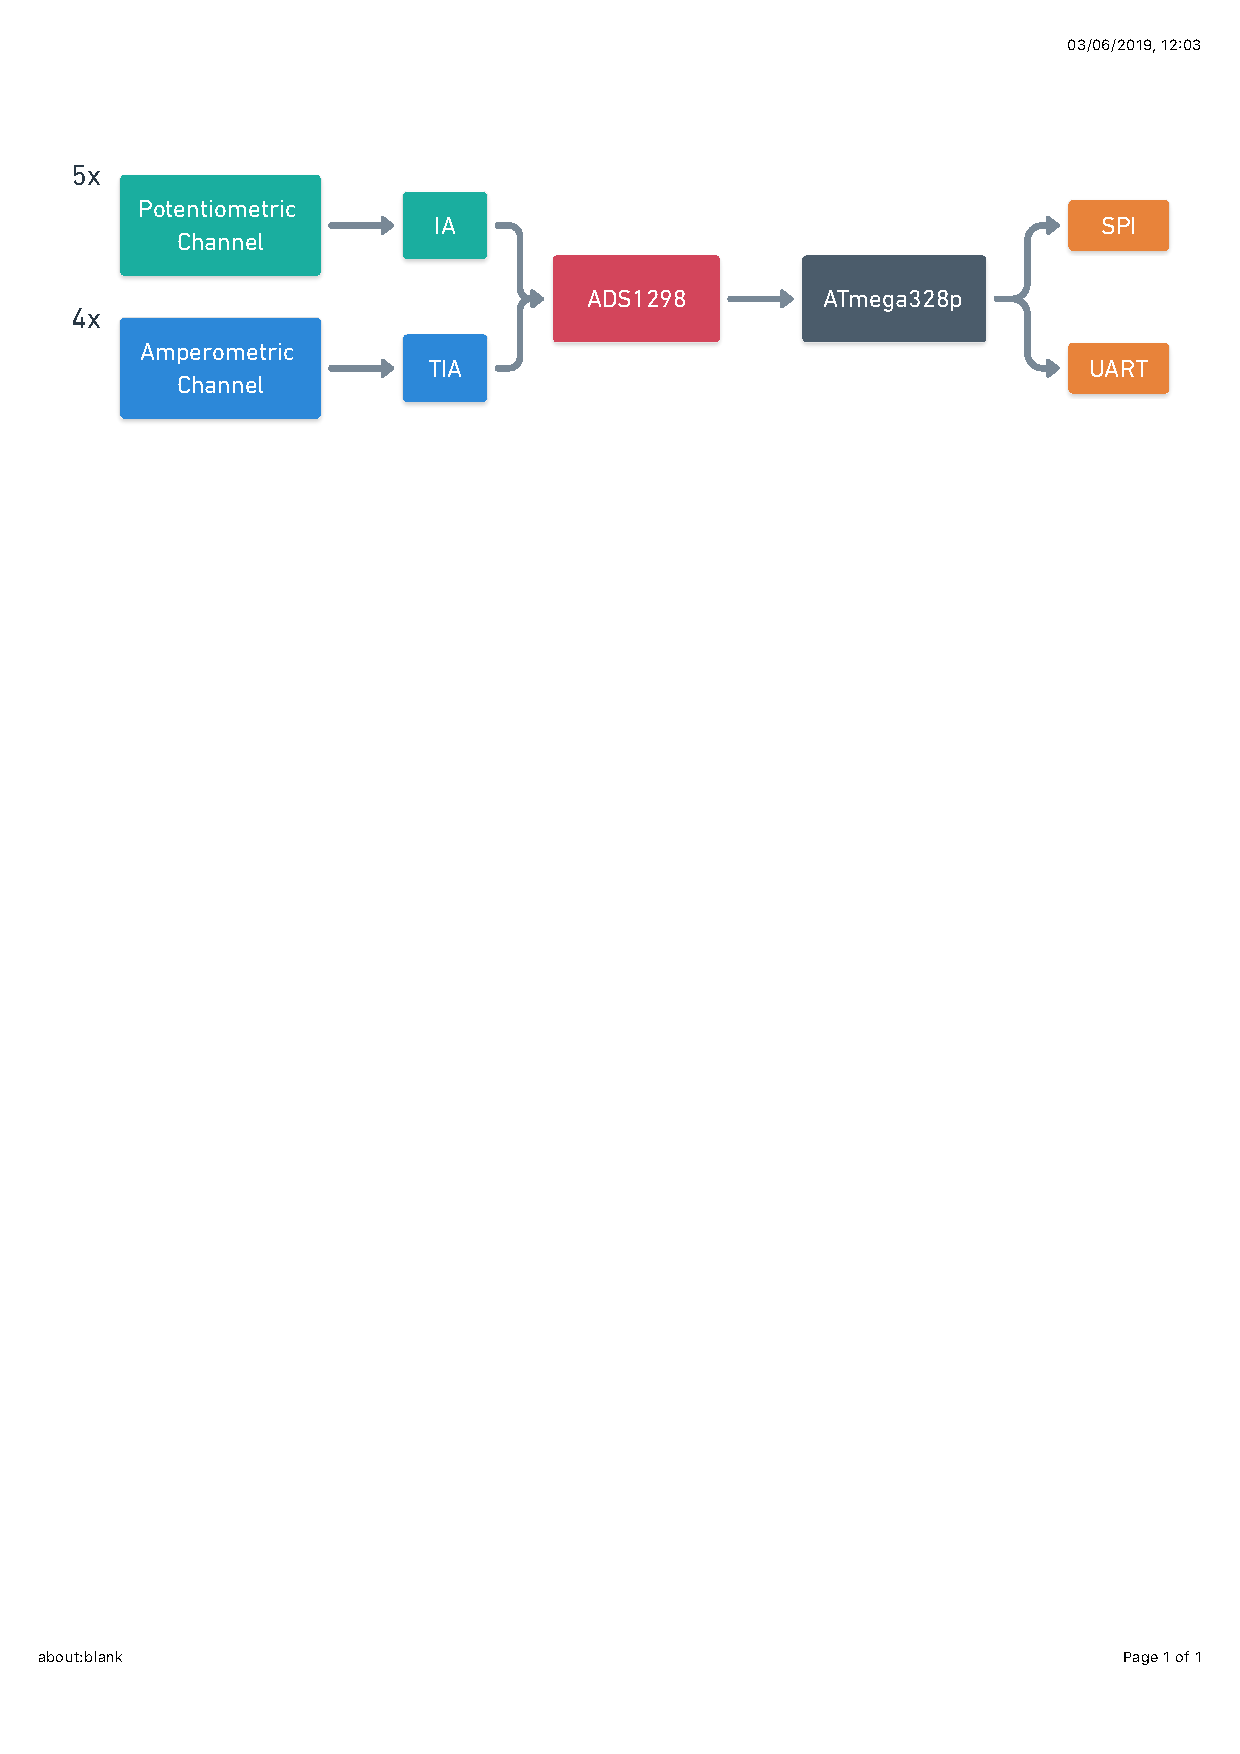
\includegraphics[trim={0cm 20.5cm 0.5cm  2.5cm}, clip, width=1\textwidth]{./figures/CircuitBlockDiagram.pdf}
\captionsetup{justification=centering}
\caption{Block Diagram of the PCB being developed by the Boutelle Research Group for continuous monitoring of TBI markers}
\label{fig: PCB block diagram}
\end{figure}


\begin{figure}[b!]
\centering
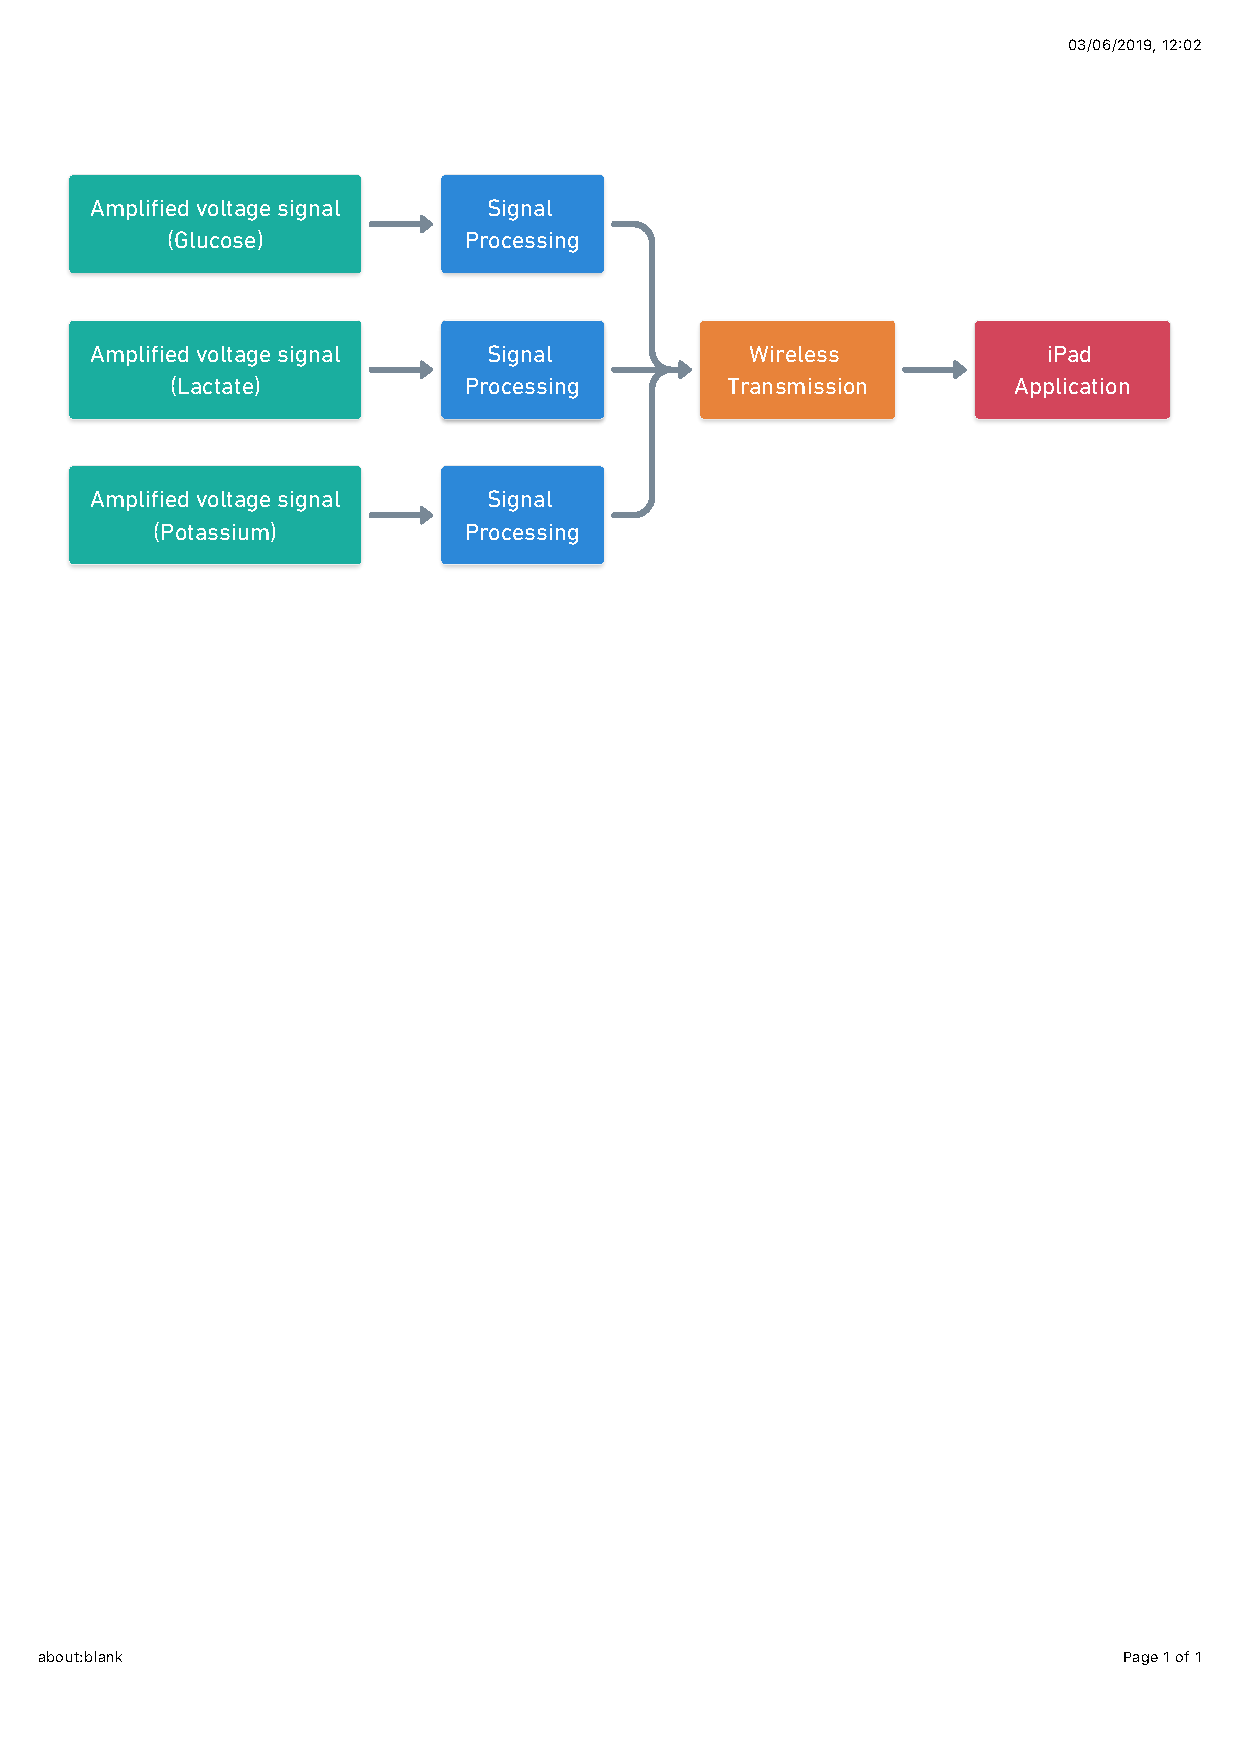
\includegraphics[trim={0cm 19.5cm 0.5cm  2.5cm}, clip, width=1\textwidth]{./figures/Flowchart.pdf}
\captionsetup{justification=centering}
\caption{Flowchart of the key elements in the prototype system}
\label{fig: flowchart}
\end{figure}

The prototype developed is a simplified model of the PCB. The prototype receives three amplified voltage signals, corresponding to glucose, lactate and potassium, so it continues on from the PCB block diagram after the ADS1298. The prototype then extends further from the functionality of the PCB by processing the received signals, developing the wireless transmission of the data and developing an iPad application, as shown in the flowchart in Figure~\ref{fig: flowchart}. The code for this project can be found in Appendix~\ref{appendix: a}.



\subsection{Hardware}
The hardware of the prototype consists of an Arduino Nano and a Adafruit Bluefruit LE SPI Friend, as shown in Figure~\ref{fig: breadboard}. The Arduino Nano was chosen as a suitable microcontroller for prototyping and mimicking the PCB as it also contains an ATmega328p microcontroller and has an inbuilt ADC. However, the ADC is only 10-bit, so it has poorer precision than the ADS1298. The Arduino is also simple to programme due to the IDE and libraries available, making it suitable for prototyping.

\begin{figure}[H]
\centering
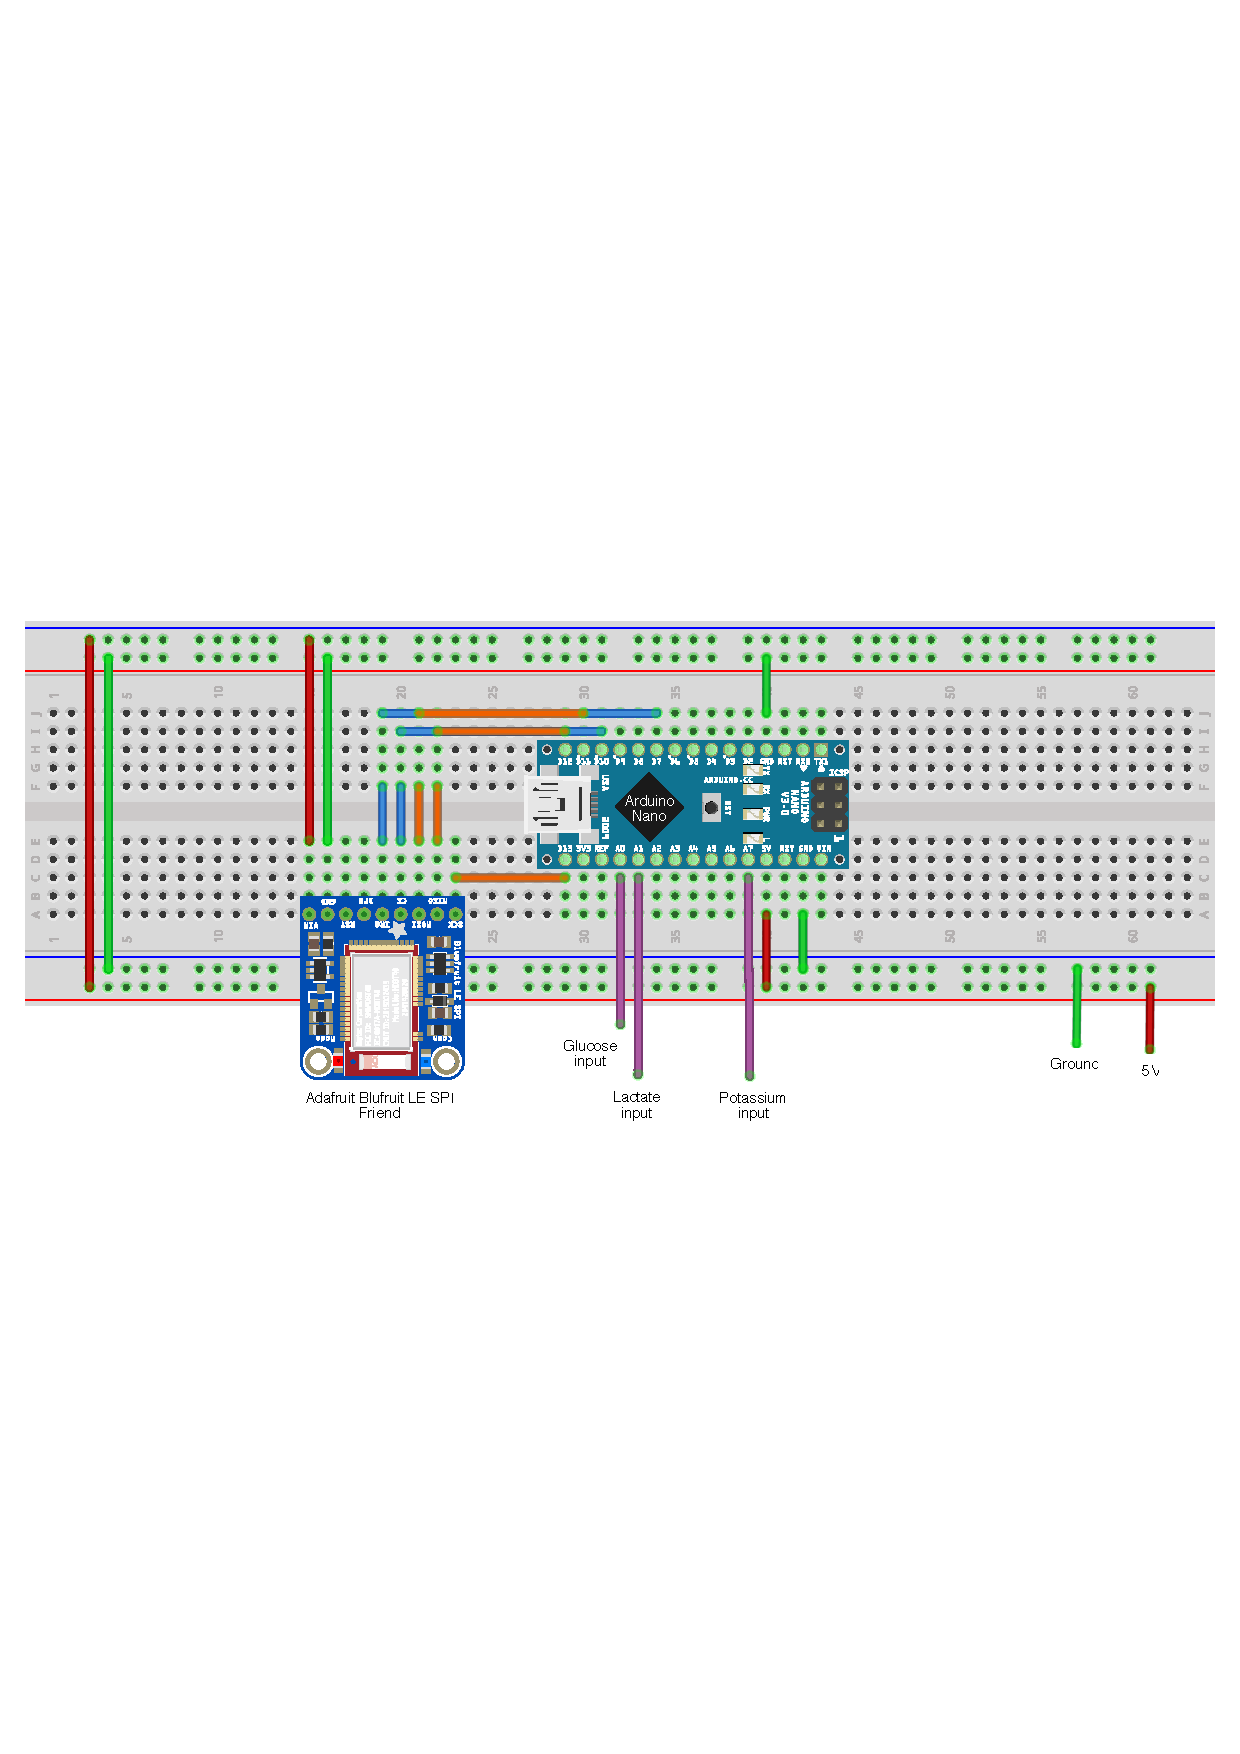
\includegraphics[trim={0cm 10.5cm 0cm  10cm}, clip, width=1\textwidth]{./figures/Breadboard2.pdf}
\captionsetup{justification=centering}
\caption{Prototype assembled on breadboard}
\label{fig: breadboard}
\end{figure}

The Arduino Nano receives three input voltage signals ranging from 0V to 5V at the analogue pins A0, A1, and A7. These input pins correspond to glucose, lactate, and potassium. The signals are discretised by the inbuilt ADC. The Nano records the time at which each signal is read, along with the value of the signal. The signal recordings are processed before being passed to the Bluefruit.



\subsection{Firmware}
The Arduino Nano is encoded to sample and process the three input signals received, then to control the Bluefruit to wirelessly transmit the signals via Bluetooth low energy (BLE). The algorithm encoded in the Arduino is described in Figure~\ref{fig: psuedocode}.


\subsubsection{Signal Processing}
Every 200ms the Arduino reads the input signals at the A0, A1 and A7 pins and records the time, in milliseconds since the Arduino was connected to power, at which sampling occurred. Each input signal received by the Arduino is filtered with a low-pass filter with a cut off frequency of 1Hz. This cut off frequency was chosen because the events indicating a SD occur over a long time frame, as shown in Figure~\ref{fig: SD}, hence the changes occur slowly and at low frequency. The low pass filter attenuates high frequency components that may arise from noise or patient movement, allowing for a cleaner signal to be obtained.

For every five samples of data recorded, so in a 1s period, the average voltage is calculated for each signal. This averaging methods allows large deviations and spikes to be smoothed, thereby reducing the effect of noise on the outputted data.

\begin{figure}[t!]
\centering
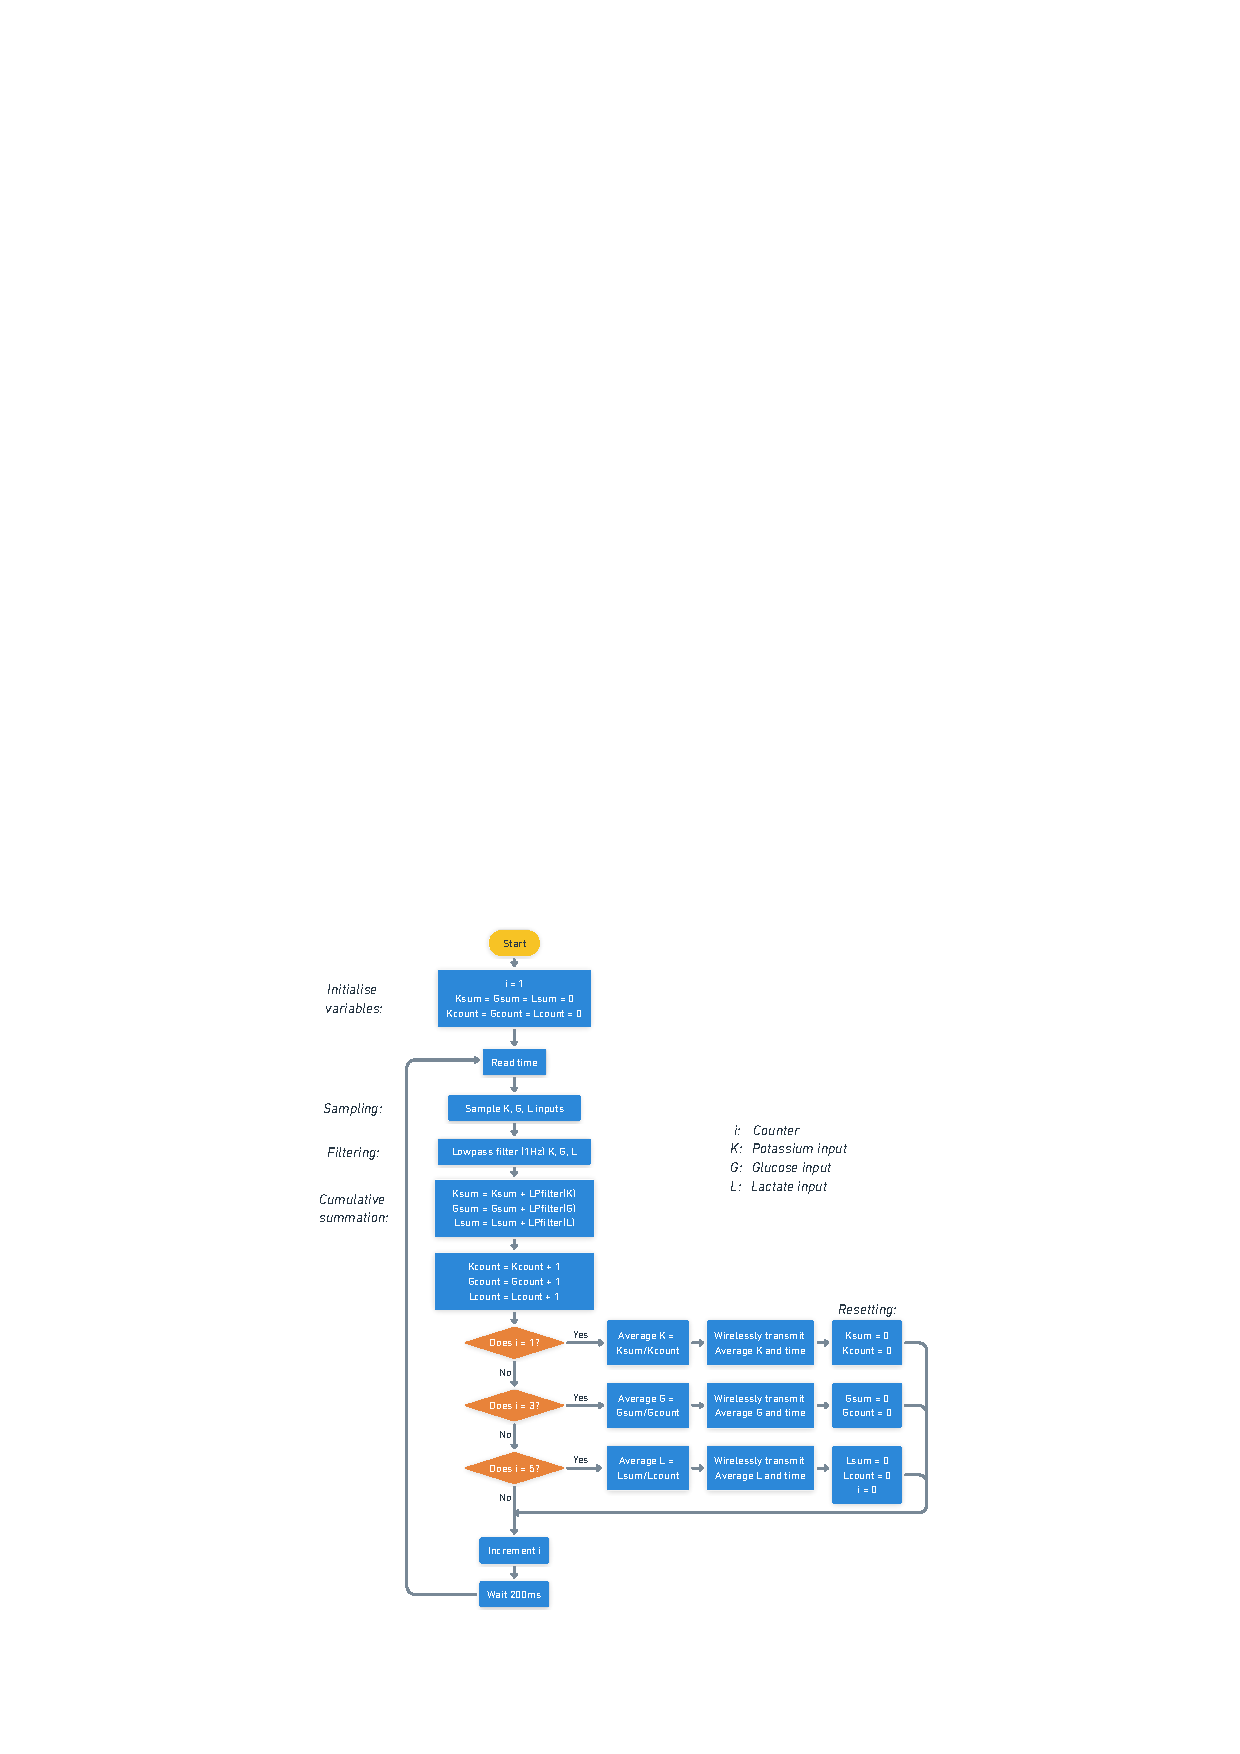
\includegraphics[trim={1cm 5cm 1cm  4cm}, clip, width=1\textwidth]{./figures/psuedocode.pdf}
\captionsetup{justification=centering}
\caption{Flowchart of algorithm encoded in Arduino Nano}
\label{fig: psuedocode}
\end{figure}



\subsubsection{Wireless Transmission}
BLE and ZigBee are both popular wireless data transmission options for IoT projects. Table~\ref{table:BLE vs ZigBee} summarises the differences between BLE and ZigBee. For this project, BLE is the most suitable option. BLE offers more efficient data transfer, shown by the lower latency time and higher throughout, and is compatible with iOS. A disadvantage of BLE is that it has a shorter range than ZigBee, however this is not of hindrance as the range is sufficient for the application since the patient will remain close to the iPad that will receive the transmitted signals. BLE is commonly used for health and fitness trackers, making it a suitable method of transmission for this project's application.

\begin{table}[h!]
\centering
\begin{tabular}{||c c||} 
 \hline
 BLE & ZigBee \\ [0.5ex] 
 \hline\hline
 Short range (77m) & Medium range (291m) \\
 Higher data rate: 1Mbps bursts & Lower data rate: 250kbps \\ 
 PAN (personal area network) & LAN (local area network) \\
 Throughput: 0.27Mbps & Throughput: 0.03Mbps \\
 Latency: 3-6ms & Latency: 15ms \\
 Sleeps between bursts $\rightarrow$ uses less power & No sleep functionality \\
 Supported on most OSs including iOS & Not supported on most OSs \\
 \hline
\end{tabular}
\caption{BLE vs. ZigBee \cite{Ray2015, Christiano}}
\label{table:BLE vs ZigBee}
\end{table}

Adafruit provide a variety of Bluetooth low energy modules that are compatible with Arduino, and they provide a library that can be used with the Arduino IDE: Adafruit\_BluefruitLE\_nRF51. Adafruit also provide an iOS app to test the bluetooth module and view the received signals. Whilst the PCB currently being developed allows for both SPI and UART data transmission, SPI was the chosen mode for the prototype hence the Bluefruit LE SPI Friend was chosen over the Bluefruit LE UART Friend. Both share similarities and use the same library in the Arduino IDE, however SPI was preferred as it has a clock line where data can be sent along with the clock pulses, so the timing of when data is sent is more reliable. The Arduino Nano has inbuilt SPI pins: D11 is MOSI, D12 is MISO and D13 is SCK. These connect to the corresponding pins on the Bluefruit, which are shown by the orange connections in Figure~\ref{fig: breadboard}. D10 on the Arduino is programmed as the CS and D7 is programmed as the IRQ, which are then wired to the corresponding Bluefruit pins, shown by the blue wires in Figure~\ref{fig: breadboard}. 

The Adafruit\_BluefruitLE\_nRF51 library provides a header file specifically for the Bluefruit LE SPI Friend which provides functions that allow for the transmission of data via BLE to a paired device. The function used is {\tt{ble.print()}}. The limitation of this function is that a maximum of 20 characters can be sent at a time otherwise the data becomes fragmented. This means that the data from each input pin and the corresponding time of recording has to be wirelessly transmitted one at a time rather than all three sent simultaneously to prevent the risk of the data fragmenting. The data from each input pin is outputted in characters as:

\begin{align}
    Output = ID + Time + Voltage + \backslash n.
    \nonumber
\end{align}

The \textit{ID} at the beginning identifies which signal is being sent i.e. G for glucose, and the newline character (\textit{$\backslash$n}) at the end concludes the the string being transmitted. If both these identifiers are not present at these specific locations when received on the app, this indicates that the data is fragmented and the app will discard the data. 

Another limitation was observed when all three inputs were periodically sent within a 200ms period. The data would initially be sent correctly but after some time, the data would fragment. The Bluefruit struggled to send the data so quickly, which created a backlog of data that was responsible for the fragmentation. Eventually, the Bluetooth module would disconnect from the app. To prevent this, the three signals were periodically sent every 1s, spaced such that potassium was sent at 200ms, glucose at 600ms, and lactate on the 1s as highlighted in Figure~\ref{fig: psuedocode}. Since the electrochemical changes in the brain occur at slow rates, for example an SD event takes about 10 minutes, a sampling speed of 1s on the app is suitable for this application. 





\subsection{iPad Application}
The iPad app was written in Swift using XCode. The app layout is shown in Figure~\ref{fig: storyboard}. The three pages shown in section 3 of Figure~\ref{fig: storyboard} all have the same layout. Details of this layout can be seen clearly on the Potassium Ion Concentration page, and the pages Glucose Concentration and Lactate Concentration have the same features. 

Once the user logs in, the app connects to the Bluefruit LE SPI Friend and receives the strings of data sent by the Bluefruit and checks that the \textit{ID} and newline character are in place. Depending on the \textit{ID}, the app stores the \textit{Time} and \textit{Voltage} string in arrays corresponding to the electrochemical signal being read, i.e. if the \textit{ID = G}, the \textit{Time} is appended to an array called  {\tt{Gtime}} and \textit{Voltage} is appended to an array called {\tt{Gvoltage}}. Each new data string for a given electrochemical signal is received every 1s. The \textit{Time} string received is converted from the time in milliseconds into the real clock time at which the signal was read from the Arduino analogue input pin. It is important that the signals are timestamped with the real time of recording as opposed to the time at which the signals were received on the app because over time there may be a time lag in transmission.

\begin{figure}[p]
\centering
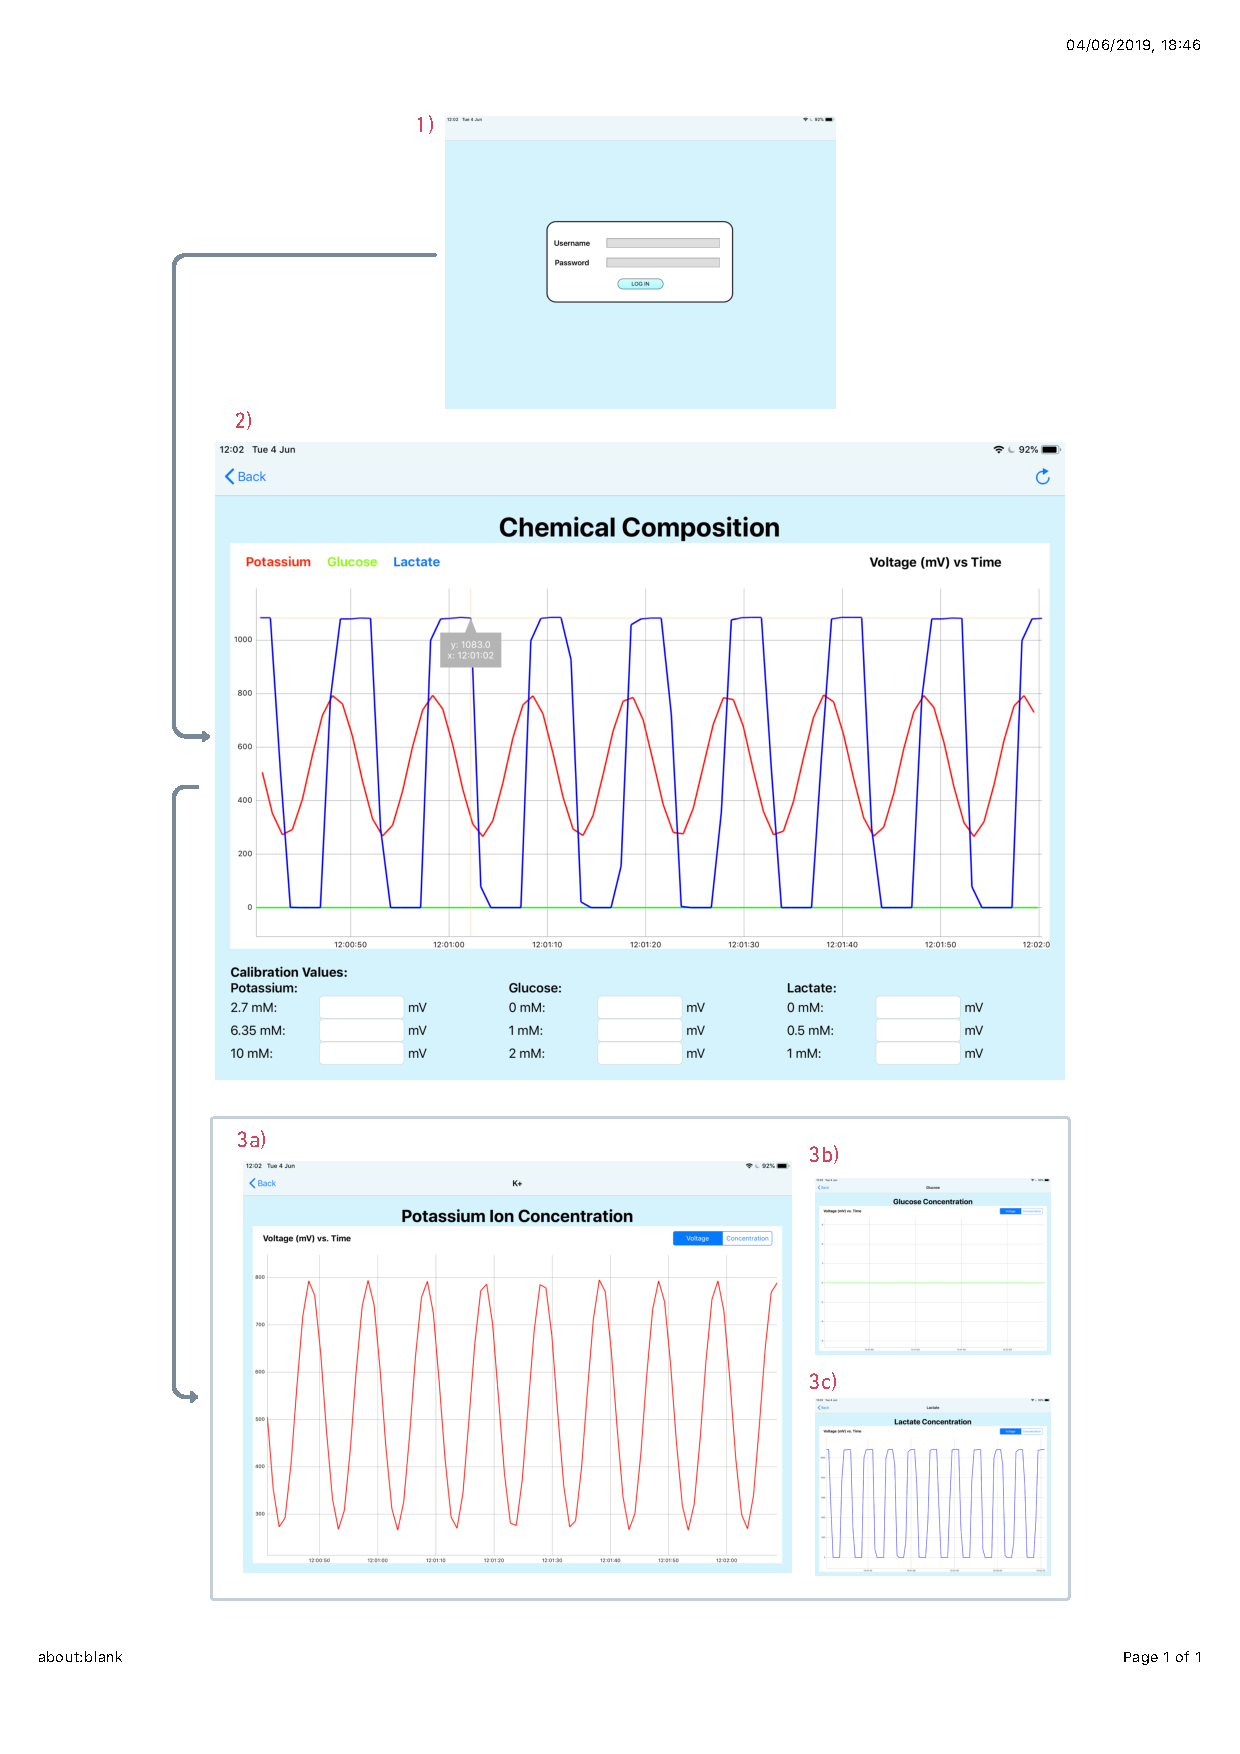
\includegraphics[trim={1cm 2.5cm 1cm  2cm}, clip, width=1\textwidth]{./figures/appStoryboard3.pdf}
\captionsetup{justification=centering}
\caption{Storyboard of the iPad application. 1) Log in page. 2) Chemical Composition page. 3a) Potassium Ion Concentration page. 3b) Glucose Concentration page. 3c) Lactate Concentration page. Pages 3a, 3b, and 3c have the same layout and are accessed from Page 2.}
\label{fig: storyboard}
\end{figure}


\subsubsection{Charts API}
To convey the information to the clinician clearly, the data received was displayed graphically using the Charts API developed by Daniel Gindi. The API allowed for basic graphs to be fully customised based on the needs of this project. The graphs display the voltage recorded from an input pin against the real clock time of the reading for each electrochemical signal. The app allows for all three signals to be viewed on one graph, as seen on the Chemical Composition page in Figure~\ref{fig: storyboard}, or as individual plots shown in pages 3a, 3b and 3c. These individual plots can be accessed by clicking on the graph legends on the Chemical Composition page, located above the graph. All graphs can be scaled and are zoombale, allowing to clearly view specific data. Furthermore, clicking on a specific point on a plot displays a grey bubble at the location which shows the corresponding x and y value at that point. This feature can be seen on the Chemical Composition page but works across all plots on all pages.


\subsubsection{Calibration}
In the individual concentration plots on pages 3a, 3b, and 3c in Figure~\ref{fig: storyboard}, in the top right corner of the graph there is a segmented control button that has \textit{Voltage} on the left and \textit{Concentration} on the right. Selecting a button allows to view the graph with either voltage or concentration on the y-axis. To convert the voltage values received into the corresponding concentration of the electrochemical signal in the brain, the relationship between the two needs to be known. This is obtained through calibration. 

\begin{table}[h!]
\centering
\begin{tabular}{||c c c||} 
 \hline
 [K+] (mM) & [Glucose] (mM) & [Lactate] (mM) \\ [0.5ex] 
 \hline\hline
 2.70 & 0.00 & 0.00 \\
 6.35 & 1.00 & 0.50 \\
 10.00 & 2.00 & 1.00 \\
 \hline
\end{tabular}
\caption{Known concentrations of solutions used for calibration}
\label{table: calibration conc}
\end{table}

During calibration, known concentrations of potassium ions, glucose and lactate, shown in Table~\ref{table: calibration conc}, are provided to the microdialysis system and the outputted voltage is recorded. Whilst monitoring a patient, calibration occurs at frequent intervals as the sensors degrade over time, hence voltage output for the same known concentration will change with time. The Chemical Composition page of the app allows for the calibration values to be typed into the text field. Once the calibration voltages have been inputted, the input voltages can be converted into concentration when the \textit{Concentration} button is clicked on the segmented control, and the graph displays concentration against real time. If calibration values aren't provided and the \textit{Concentration} button is clicked, the app will prompt the user to insert the calibration voltages on the Chemical Composition page. \newline 

\noindent \underline{Potassium Calibration} 

For potassium, the conversion from voltage to concentration is given by a logarithmic relationship and can be derived by considering an ion selective electrode. \textbf{** NEED TO COMPLETE **} \newline 

\noindent \underline{Glucose and Lactate Calibration} 

The conversion from voltage to concentration for glucose and lactate is derived from the enzymatic catalysed reaction that occurs on the electrode surface of the sensors \cite{Patel:2011:10.1016/j.bios.2010.11.033}, and can be obtained by starting from the Hill equation. Since the sensors measure current, the Hill equation is written as

\begin{equation}
    I_{rate} = \frac{I_{max}}{1 + \big( \frac{K_{m}}{[S]} \big)^{n}},
    \label{equation: Hill equation}
\end{equation}

\noindent where $I_{rate}$ is the reaction rate, $I_{max}$ is the maximum reaction rate, $[S]$ is the substrate concentration, i.e. glucose or lactate concentration, $K_{m}$ is the substrate concentration that results in a rate that is $\frac{I_{max}}{2}$, and $n$ is the Hill coefficient which is a measure of cooperativity between the substrate and binding site.

The Hill coefficient is equal to 1 since glucose and lactate have no substrate binding cooperativity. Therefore the Hill Equation can be reduced to the Michaelis-Menten equation, which is given by:

\begin{equation}
    I_{rate} = \frac{I_{max}[S]}{[S] + K_{m}}.
    \label{equation: Michaelis_menten}
\end{equation}

Since the concentrations of glucose and lactate being measured is low, such that $[S] << K_{m}$, equation~\ref{equation: Michaelis_menten} is reduced to a linear equation:

\begin{equation}
    I_{rate} = \frac{I_{max}[S]}{K_{m}}.
    \label{equation: reduced Michaelis_menten}
\end{equation}

\noindent Since the transimpedance amplifier converts the current to voltage, the relationship between voltage and concentration is a linear in the form of $y = mx + c$.

During calibration, only three known concentrations of solutions are used and the corresponding voltages recorded. Having few data points reduces the accuracy of the linear equation that best fits through the data points. Furthermore, there are numerous lines of best fit that would fit the data. Therefore, the optimal line of best fit can be found using least squares regression:

\begin{equation}
    m = \frac{ \sum_{i=1}^{3} \big( x_{i} - \Bar{X} \big) \big( y_{i} - \Bar{Y} \big) }{ \sum_{i=1}^{3} \big( x_{i} - \Bar{X} \big)^{2} },
    \label{equation: least squares regression}
\end{equation}
\begin{equation}
    c = \Bar{Y} - m\Bar{X},
\end{equation}

\noindent where $x_{i}$ is voltage recording, $\Bar{X}$ is the average voltage recording, $y_i$ is the known concentration, and $\Bar{Y}$ is the average concentration from the data set. 

Now that the $m$ and $c$ coefficients have been determined, using $Concentration = m*Voltage + c$ the plot of voltage vs. time can be transposed into concentration vs. time for glucose and lactate.


% K+ derivation




\newpage

\section{Testing}
\subsection{Standard Signals}
% describe testing procedure done in labs
% mention limitation of picoscope so had one constant signal connected to Arduino GND pin. Fixed voltage

% purpose of the test is to show the app can receive three signals simultaneously, compare the signals with expected values on PicoLab, and show features of the app. evaluate suitability of filtering and averaging

\subsection{Brain Signals}
\newpage

\section{Results}
% do i need subsections?

\subsection{Standard Signals}
% Insert plots comparing PicoLog and on app
% comment on shape, peak to peak voltage etc. 
% comment on peak time i.e. if there is a lag 
% able to do three curves at once

% comment on each wave.
% - sine wave is relatvely well represented
% - lower freq sine wave performs better? more points in a period are sampled?
% - sqaure wave has discontinutites. there aren't representd as well. Expand on this point in the DISCUSSION saying that even though this is the case, the sudden disconitnuities tend to be noise and electrical artifacts. the transient changes occur gradually, and as shown by the sin wave will be able to be captured

\subsection{Brain Signals}
\newpage

\section{Discussion}
\subsection{Standard Signals Test}

From the experiments, the sine waves produced on the app were well represented compared to those produced on the PicoLog. The sine wave with a lower frequency held its shape better on the app as more points on the sine wave could be sampled as the signal frequency was much less than the app's sampling frequency of 1s. 

On the other hand, the squares wave's discontinuities were not as sharp on the app compared to the PicoLog. This is due to the averaging method implemented on the Arduino. The Arduino reads in five input signal per second and the mean value is calculated and sent to the app. When a sharp discontinuity occurs, the averaging method softens this sudden change. Whilst the square wave cannot be replicated exactly, this issue doesn't affect the neurochemical signals. As seen in Figure~\ref{fig: SD}, any sharp discontinuities that occur are due to noise or electrical artefacts, so the averaging method implemented will smooth out these. The transient changes that occur during an SD for potassium, glucose and lactate occur gradually so the shape will be able to be captured.

% relate the above paragraph to testing with real signals if it shows what i have written.

% mention time lag 

\subsection{Spreading Depolarisation}

\subsection{Limitations and Future Improvements}


\newpage



%\section{Acknowledgements}
%I would like to thank Professor Martyn Boutelle for allowing me to pursue this project that has greatly diversified my skill set, and for guiding me through this project. I would also like to thank Dr. Michelle Rogers for helping me navigate through LabChart and understanding the data. I would like to thank Aidan Wickham for providing me with details about his PCB, which this project is based on. I would also like to thank Georgios Zafeiropoulos and Konstantinos Petkos for guiding me through the best methods to validate and test my prototype. 

%Finally, I would like to thank my parents, Dr. Jayaprakash Pattar and Dr. Jyothsna Murthy, for believing in me more than I could ever believe in myself, and Rohan Padmanabhan for always supporting me through the highs and lows of this project.

%\newpage
\bibliography{library.bib}
\bibliographystyle{unsrt}

%\newpage

%\appendix

%\section{Appendix: Project Code}
%\label{appendix: a}
%\begin{itemize}
%    \item Firmware code can be found at: \newline \url{https://github.com/ajp15/MEngIndvProject-arduino}
 %   \item iPad app development can be found at: \newline \url{https://github.com/ajp15/MEngIndvProject-app2}
%\end{itemize}


\end{document}
